\documentclass[%
12pt, %
final, % 
oneside, % 
onecolumn, %  
centertags]{article} % относится к классу article и размер шрифта 12 пунктовб, {article: статья, report: отчеты и диссертации, book: книга, letter: письмо}

% \usepackage{fontspec}
 
% \setmainfont{Times New Roman}

% \documentclass[a4paper, 12pt]{report}

\topmargin= -30pt % насколько сверху будет страница
\textheight= 650pt


\usepackage[utf8]{inputenc} % задает кодировку, utf-8 кодировка, включающая в себя знаки почти всех языков мира
\usepackage[english]{babel} % подключает необходимые языки, основным языком является английский

\selectlanguage{english} % настройки будут на английском, но писать будет на русском

\usepackage{euscript}
\usepackage{supertabular}

\renewcommand{\baselinestretch}{1.0} 

\usepackage[colorlinks=true,linkcolor=blue,unicode=true,urlcolor = blue]{hyperref} %hypered
\usepackage[pdftex]{graphicx} % для графики

\usepackage{amsthm, amssymb, amsmath, amsfonts} % математический пакет, математические шрифты
\usepackage{textcomp}
\usepackage[noend]{algorithmic}
\usepackage[ruled]{algorithm}
\usepackage{lipsum}
\usepackage{indentfirst}
\usepackage{babel}
\usepackage{pgfplots}
\usepackage{setspace}
\usepackage{xcolor}
\usepackage{hyperref}
\usepackage{subfigure}

\setcounter{secnumdepth}{5}
\setcounter{tocdepth}{5}
\newcommand\simpleparagraph[1]{%
  \stepcounter{paragraph}\paragraph*{\theparagraph\quad{}#1}}
\usepackage{listings}
% \usepackage{xcolor}
%\usepackage{minted}

\lstset { %
     language=C++,
     backgroundcolor=\color{black!5}, % set backgroundcolor
     basicstyle=\footnotesize,% basic font setting
}


\linespread{1.0} 
\setlength{\parindent}{2.4em}
\setlength{\parskip}{0.1em}

\pgfplotsset{compat=1.9}
\pgfplotsset{model/.style = {blue, samples = 100}} 
\pgfplotsset{experiment/.style = {red}}

\theoremstyle{plain}
\binoppenalty=10000

\newtheorem{theorem}{Theorem}[section] % theorem

\theoremstyle{definition}
% \newtheorem{definition}{Определение}[subsection]
\newtheorem{definition}{Definition}[subsection]

\theoremstyle{remark}
% \newtheorem{remark}{Замечание}[section]

% \newtheorem{corollary}{Следствие}

% \newtheorem{proposition}{Proposition}

% \newtheorem{example}{Пример}

% \newtheorem{lemma}{Лемма}[section]

\renewcommand*{\proofname}{Proof}

\graphicspath{ {./images/} }


% \usepackage{amsmath,amsfonts,amssymb, setspace}  % Разнообразные математические команды и значки
% \usepackage{indentfirst}     % Отступ в первом абзаце

% \pagestyle{empty}
\usepackage[left=2.5cm, right=1.5cm, top=2.5cm, bottom=2.5cm]{geometry}
\usepackage[medium]{titlesec}
\usepackage{graphicx}
% \graphicspath{ {./images/} }

\begin{document}

	\begin{titlepage} 
		\begin{center}
		\textbf{}\\[2.0cm]
		\LARGE \ \\[0.5cm]
		\Large \  \\[3cm]
		\LARGE Probability test


		\begin{flushright}
		Performed by\\
		Aleksandr Shirokov\\

		\end{flushright}

		\vfill 

		{\Large {St. Petersburg}} \par
		{\Large {2021}}
		\end{center} 
	\end{titlepage}

\tableofcontents
\newpage


\section{Tasks}


\subsection{Task 1}

\begin{center}
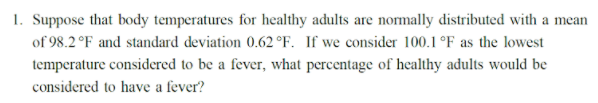
\includegraphics[scale=0.9]{1.png}
\end{center}

\textbf{Answer}: normally distibution $\xi \sim N(98.2, 0.62)$. $X_1 = 100.1$, $\xi = 0.62\nu + 98.2$, $\nu \sim N(0, 1) = \frac{\xi - 98.2}{0.62}$

$$P\left(\xi \leq X_1 \right) = P\left(\frac{\xi - 98.2}{0.62} \leq \frac{100.1 - 98.2}{0.62}\right) = \Phi_{\nu}(3.06) = 0.9989$$

So the answer of percentage of healthy adults would be considered tohave a fever is $1 - 0.9989 = 0.001$ or $0.1$ percent

\subsection{Task 2}

\begin{center}
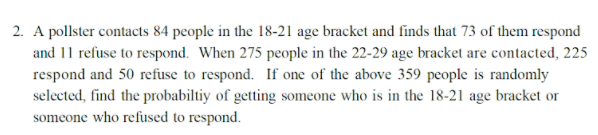
\includegraphics[scale=0.9]{2.png}
\end{center}

\textbf{Answer}: 

We can select one of people from $18-21$ (first probability) or one from people who refuse to respond ($20$ from second group):

$$\frac{84}{359} + \frac{50 + 11}{359} - \frac{11}{359} = \frac{134}{359}$$

\subsection{Task 3}

\begin{center}
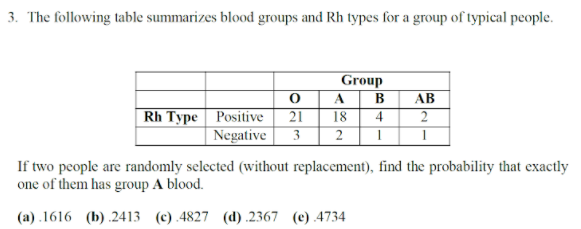
\includegraphics[scale=0.9]{3.png}
\end{center}

\textbf{Answer}: the mutiplication of probabilites with $A$ group and not $A$:

$$C_2^1 \cdot \frac{20}{52} \cdot \frac{32}{52} = 0.4734$$

Answer $E$

\subsection{Task 4}

\begin{center}
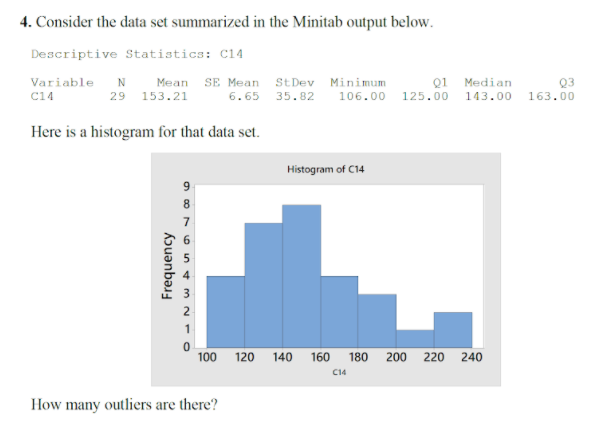
\includegraphics[scale=0.9]{4.png}
\end{center}

\textbf{Answer}: data is not in normal distribution so for outliers we will use interquantile method to find outliers:

$$IQR = Q_3 - Q_1 = 163 - 125 = 38$$

$$(Q_1 - 1.5IQR, Q_3 + 1.5IQR) = (68, 220)$$

So the outliers are more than $220$ and less than $68$. For less than $68$ there is no data, but for $220$ there are two values. Answer: \textbf{2} outliers.




\subsection{Task 5}

\begin{center}
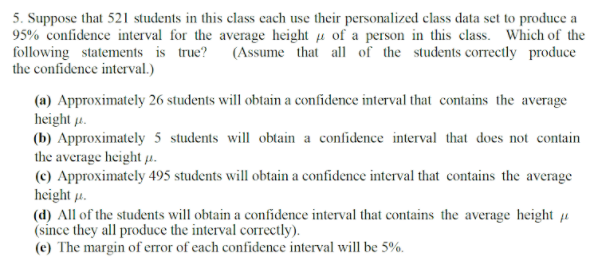
\includegraphics[scale=0.9]{5.png}
\end{center}

Answer $d$ looks right.

\end{document}